\documentclass[conference]{IEEEtran}

\usepackage{amsmath}
\usepackage{graphics}
\usepackage{graphicx}
\usepackage[english]{babel}

\bibliographystyle{/home/rsheissa/papers/midwest/IEEEtran}

\begin{document}

% paper title
\title{A CAD Tool for Automated Bandwidth Design of Negative Feedback Amplifiers}

\author{\authorblockN{Roberto Casta\~neda-Sheissa, Arturo Sarmiento-Reyes, Luis Hern\'andez-Mart\'inez and Hector V\'azquez-Leal}
\authorblockA{National Institute for Astrophysics, Optics and Electronics\\
Electronics Department, CAD Group\\
P.O. Box 51, 72000 Puebla, Pue., Mexico\\Email: rsheissa@inaoep.mx, jarocho@inaoep.mx, luish@inaoep.mx, hleal@inaoep.mx}}


% make the title area
\maketitle

\begin{abstract}
Structured design has raised as an alternative to the traditional and design approach. In the structured design, the process starts by establishing the ideal solution, which obviously fulfills a set of specifications. Hereafter, the design procedure consists in achieving a series of modifications to the ideal solution until the specs are met.

One of the key topics in the design of amplifiers is to reach a desired bandwidth (BW). This work focuses on the automation of BW design for negative feedback amplifiers through the synthesis of the nullor with active devices based on the guidelines provided by structured design.
\end{abstract}

\section{Introduction}
The design of analog amplifiers has often been considered as an art under the assumption that no systematic procedures or methodologies do exist developed so far. Experience has been the major way to produce knowledge regarding analog design. A new way to perform analog design has been developed in recent years and it has been in constant upgrade, it is called {\it structured design} \cite{verhoeven}. Herein, the main idea behind the design of negative feedback amplifiers is to divide the whole design into two main blocks, one block is the feedback network and the other block is the active part of the amplifier. As for the feedback network it is comprised of passive elements like resistors, capacitors, inducers or a combination of them.

The nullor (Figure \ref{fig:nullor}) constitutes the active (ideal) block of the amplifier. The nullor is a two-port device composed by two elements: the nullator connected at the input port and the norator connected at the output port. The transmission matrix of the nullor is composed of zeros (Eq. \ref{eq:abcd}), which indicates that the nullor possesses infinite gains for the four transfer relationships, namely voltage ($\mu$), current ($\beta$), trans-conductance ($\gamma$), and trans-impedance ($\zeta$). Since the nullor is an ideal element it is necessary to achieve its synthesis with an active device, such as BJT or MOS transistors.

\begin{equation}\label{eq:abcd}
{K}
=
\left [ \begin{array}{cc}
\frac{1}{\mu}& \frac{1}{\gamma} \\\\
\frac{1}{\zeta}& \frac{1}{\beta}
\end{array}
\right ]
=
\left [ \begin{array}{cc}
0 & 0 \\ 0 & 0
\end{array}
\right ]
\end{equation}

\begin{figure}[hbtp]
	\centering
	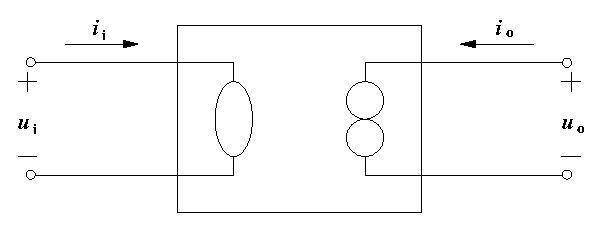
\includegraphics[scale=.7]{figures/fig_nullor.eps}
	\caption{The nullor.}
	\label{fig:nullor}
\end{figure}

The design resorts to the concept of open-loop gain-poles product \cite{verhoeven}, which is used to determine whether or not the circuit has the capability to reach the desired BW  because a flat frequency response is desired for the BW, the poles of the circuit must lie in a Butterworth distribution (Figure \ref{fig:second_butterworth}). This is done by using some well-known compensation schemes, such as pole-splitting, phantom zero, resistor broad-banding, or pole-zero cancellation. The paper presents a CAD tool that automates the BW design of negative feedback amplifiers.

\begin{figure}[hbtp]
	\centering
	\includegraphics[scale=.7]{figures/second_ord_butterworth.eps}
	\caption{Poles of the second-order Butterworth transfer function.}
	\label{fig:second_butterworth}
\end{figure}


\section{Nullor-Based Amplifiers}
On the highest design level if a passive feedback network is connected to the nullor a basic one-loop amplifier is obtained, as seen on Figure \ref{fig:one_loop}.

\begin{figure}[hbtp]
	\centering
	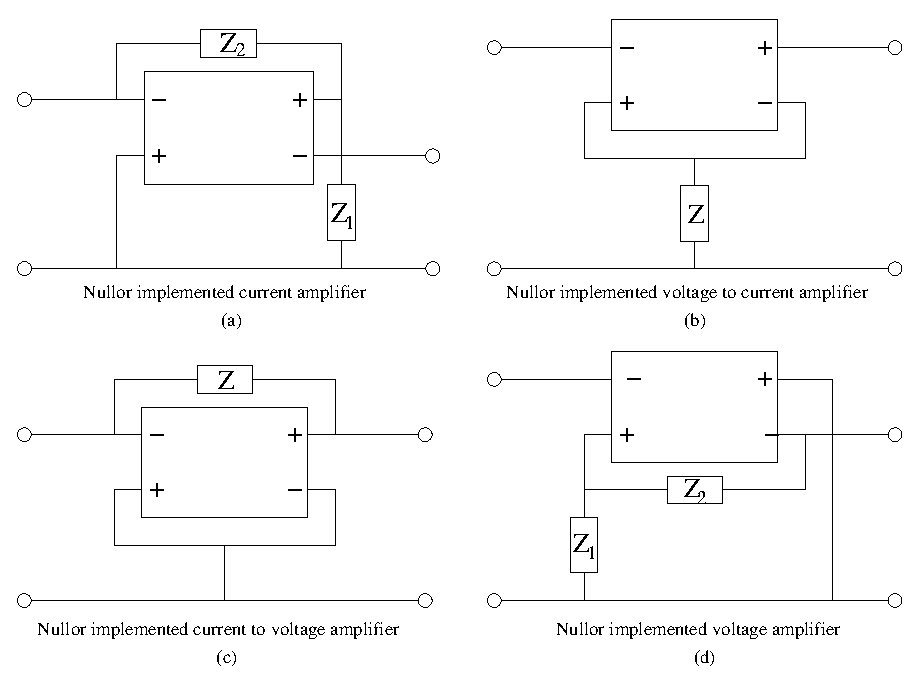
\includegraphics[scale=.5]{figures/nullor_grouped_1.eps}
	\caption{One-loop Negative-feedback Amplifiers.}
	\label{fig:one_loop}
\end{figure}
 
When one-loop amplifiers are combined, it is possible to generate two-loop amplifiers as shown in Figure \ref{fig:two_loop}. The combination of voltage amplifier and current amplifier are referred as the {\bf two-loop topology (A)} and the combination of transconductance and transimpedance amplifiers are denoted as the {\bf two-loop topology (B)} \cite{nordholt,stoffels}.

\begin{figure}[hbtp]
	\centering
	\includegraphics[scale=.5]{figures/basic_two_loops.eps}
	\caption{Two-loop Negative-feedback Amplifiers.}
	\label{fig:two_loop}
\end{figure}

Topology (B) can achieve all four kinds of transfers (voltage, current, transconductance and transimpedance), while Topology (A) can achieve all but the transconductance.

On systems design by conventional procedures designer attempts to satisfy all requirements by the judicious repeat of trial and error method. When the system is completely designed, it is verified in order to assure that complies all the function requirements, in case it fails, the design process is repeated adjusting some parameter values or modifying the configuration until all specs are accomplished \cite{ogata}.

The nullor synthesis is achieved by dividing this block into three stages to be designed:  noise, distortion and bandwidth as shown in Figure \ref{fig:block}. The noise stage is always located at the input since the noise behavior of the first stage of the active circuit is of importance. Distortion is located at the output. During these optimizations bandwidth is not taken into account. The contributions of the first and last stage to the bandwidth are taken for granted during bandwith optimization. They are taken into account, but in principle not changed.

\begin{figure}[hbtp]
	\centering
	\includegraphics[scale=.7]{figures/blocks.eps}
	\caption{Nullor synthesis.}
	\label{fig:block}
\end{figure}

As for the bandwidth behavior it is necessary to measure the bandwidth capability of the amplifier before starting the design of this last stage. This measure can be performed in a simple way using a method called Loop-gain-Poles product (LP product). When the LP product is too low (this depends on the specified bandwidth), the design can not reach the desired bandwidth. It is assumed that an all pole Butterworth characteristic is desired \cite{chen}. When the LP product is considered large enough now the placement of the poles is of concern. This is called frequency compensation. The frequency compensation techniques are not allowed to deteriorate the former design steps, i.e. noise and distortion.

\section{Program Structure}
This program uses Maple \cite{maple1, maple2} in order to perform symbolic calculations and then substitute numerical values. The program structure is based on the diagram in Figure \ref{fig:flow_diagram}.

\begin{figure}[hbtp]
	\centering
	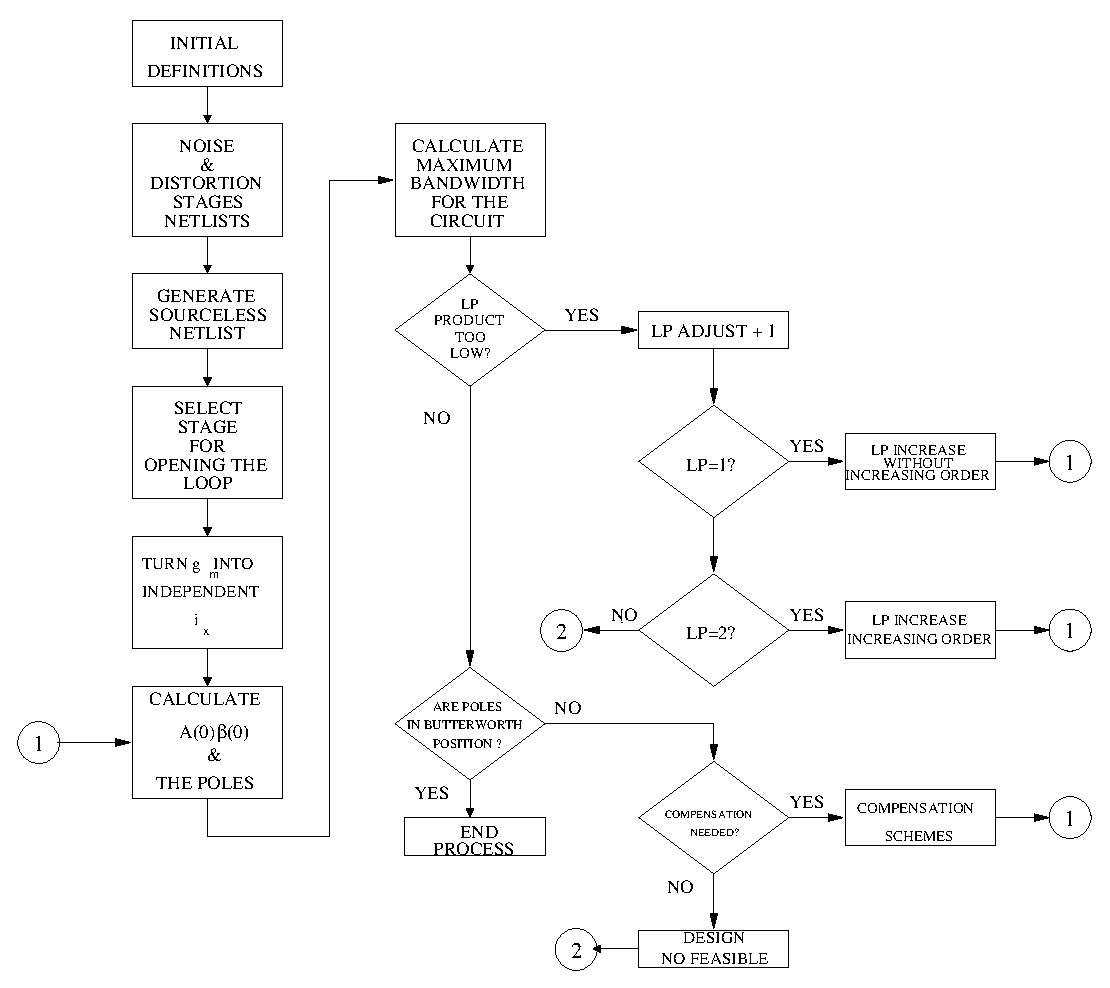
\includegraphics[scale=.5]{figures/bw_flow_diagram.eps}
	\caption{Bandwidth Program Flow Diagram.}
	\label{fig:flow_diagram}
\end{figure}

From this diagram it can be seen that the noise and distortion stages {\bf must} be already designed in order to continue the bandwidth design process. Next, a new netlist is generated with the already elements but independent sources are not included. Following this step is necessary to find the open-loop system gain by converting a controlled source to an uncontrolled one, this is done by using the sourceless netlist and selecting the stage where is more appropriate to open the loop. 

First choice is to open loop at the input stage (noise), but if this stage is comprised by devices in differential configurations the next option is the output stage (distortion). In case both stages are made of differential configurations then a common emitter in differential configuration is the last option.

Once a right controlled source is found then it is turned into an independent current source named ({\it $\text{i}_{\text{x}}$}). Afterwards, the DC-loop gain is computed as well as the poles. In order to find the poles and DC gain, Chain-matrix calculations are performed to find the MNA matrix taking as input port the port where is ({\it $\text{i}_{\text{x}}$}) and the output port is the controlling branch for the controlled source. The denominator of the found equation for this circuit gives the poles, while making s=0 gives the DC-loop gain.  Using the formula (\ref{eq:lp_prod}) the LP product is calculated, this value indicates the maximal attainable bandwidth that circuit can achieve. 

\begin{equation}\label{eq:lp_prod}
f_{n_{max}}=\sqrt[n]{\Biggl|[1-A(0)\beta(0)]\prod_{i=1}^np_i\Biggr|}
\end{equation} 

Where $A(0)\beta(0)$ is the DC loop gain and $p_i$ are system's poles. If the maximum bandwidth computed from the LP product fulfills the bandwidth requirement provided by the user the routine is stopped and the program continues to verify the position of circuit's poles. If this value is too low then a routine is performed in order to increase the LP product by already found routines \cite{verhoeven}, \cite{nordholt}. 

The first one is to increase the LP product without increasing the order, that is, increasing bias values for the noise and distortion stages. In case the LP product is not increased adjusting bias values, the other option is to increase LP value by increasing the order. This is done adding another device, care must be taken on the configuration for this device because the negative feedback must remain. If after the addition of one or more devices to this stage the LP product is still low, then the design is not feasible and must be re-designed, afterwards program ends.

Granted that the circuit is capable to achieve a desired bandwidth, the next step is to design the way how the circuit is going to do it. Now the poles placement is of concern. This is called frequency compensation. Techniques for frequency compensation are not allowed to deteriorate the noise and distortion qualities already designed.

First thing to do is locate the poles position, the important ones are placed on the left side of the real axis. The poles placement adjustment is performed by on this order: phantom zeros, pole splitting, pole-zero cancellation and resistive broad-banding. 

In case that by any of the previous compensation techniques closed-loop poles can not be placed on a Butterworth position, the design is not feasible and it is necessary to re-design it.

\section{Example}
The circuit under test is a transimpedance amplifier, that is, a current to voltage amplifier (Figure \ref{fig:one_loop} (c)). It is based on the exercise 9 of \cite{verhoeven}.

At this point the nullor has been synthesized to fulfill the noise and distortion requirements by a single CE-stage, this has been done in order to guarantee a negative loop gain (Figure \ref{fig:transimp_1}).

\begin{figure}[hbtp]
	\centering
	\includegraphics[scale=.45]{figures/transimp_1.eps}
	\caption{Transimpedance Amplifier with a Two-stage Nullor Implementation.}
	\label{fig:transimp_1}
\end{figure}

Using the small-signal model for the device, it turns to the scheme shown in Figure  \ref{fig:transimp_2}. The small-signal parameters for the device are:

\begin{itemize}
\item $g_m=40\text{mA/V}$
\item $c_{\pi}=4\text{pF}$
\item $r_{\pi}=2.5\text{k}\Omega$
\item $r_o=50\text{k}\Omega$
\item $\beta=100$
\end{itemize}

The values for the other components are as follows:

\begin{itemize}
\item $C_s=100\text{pF}$
\item $R_s=10\text{k}\Omega$
\item $R_{feed}=10\text{k}\Omega$
\item $R_L=10\text{k}\Omega$
\item $C_L=10\text{pF}$
\end{itemize}

\begin{figure}[hbtp]
	\centering
	\includegraphics[scale=.45]{figures/transimp_2.eps}
	\caption{Detailed Small-signal diagram of the amplifier of Fig.
	\ref{fig:transimp_1}.}
	\label{fig:transimp_2}
\end{figure}

The Chain-matrix for this circuit is given in Figure \ref{fig:maple_1}.

\begin{figure}[hbtp]
	\centering
	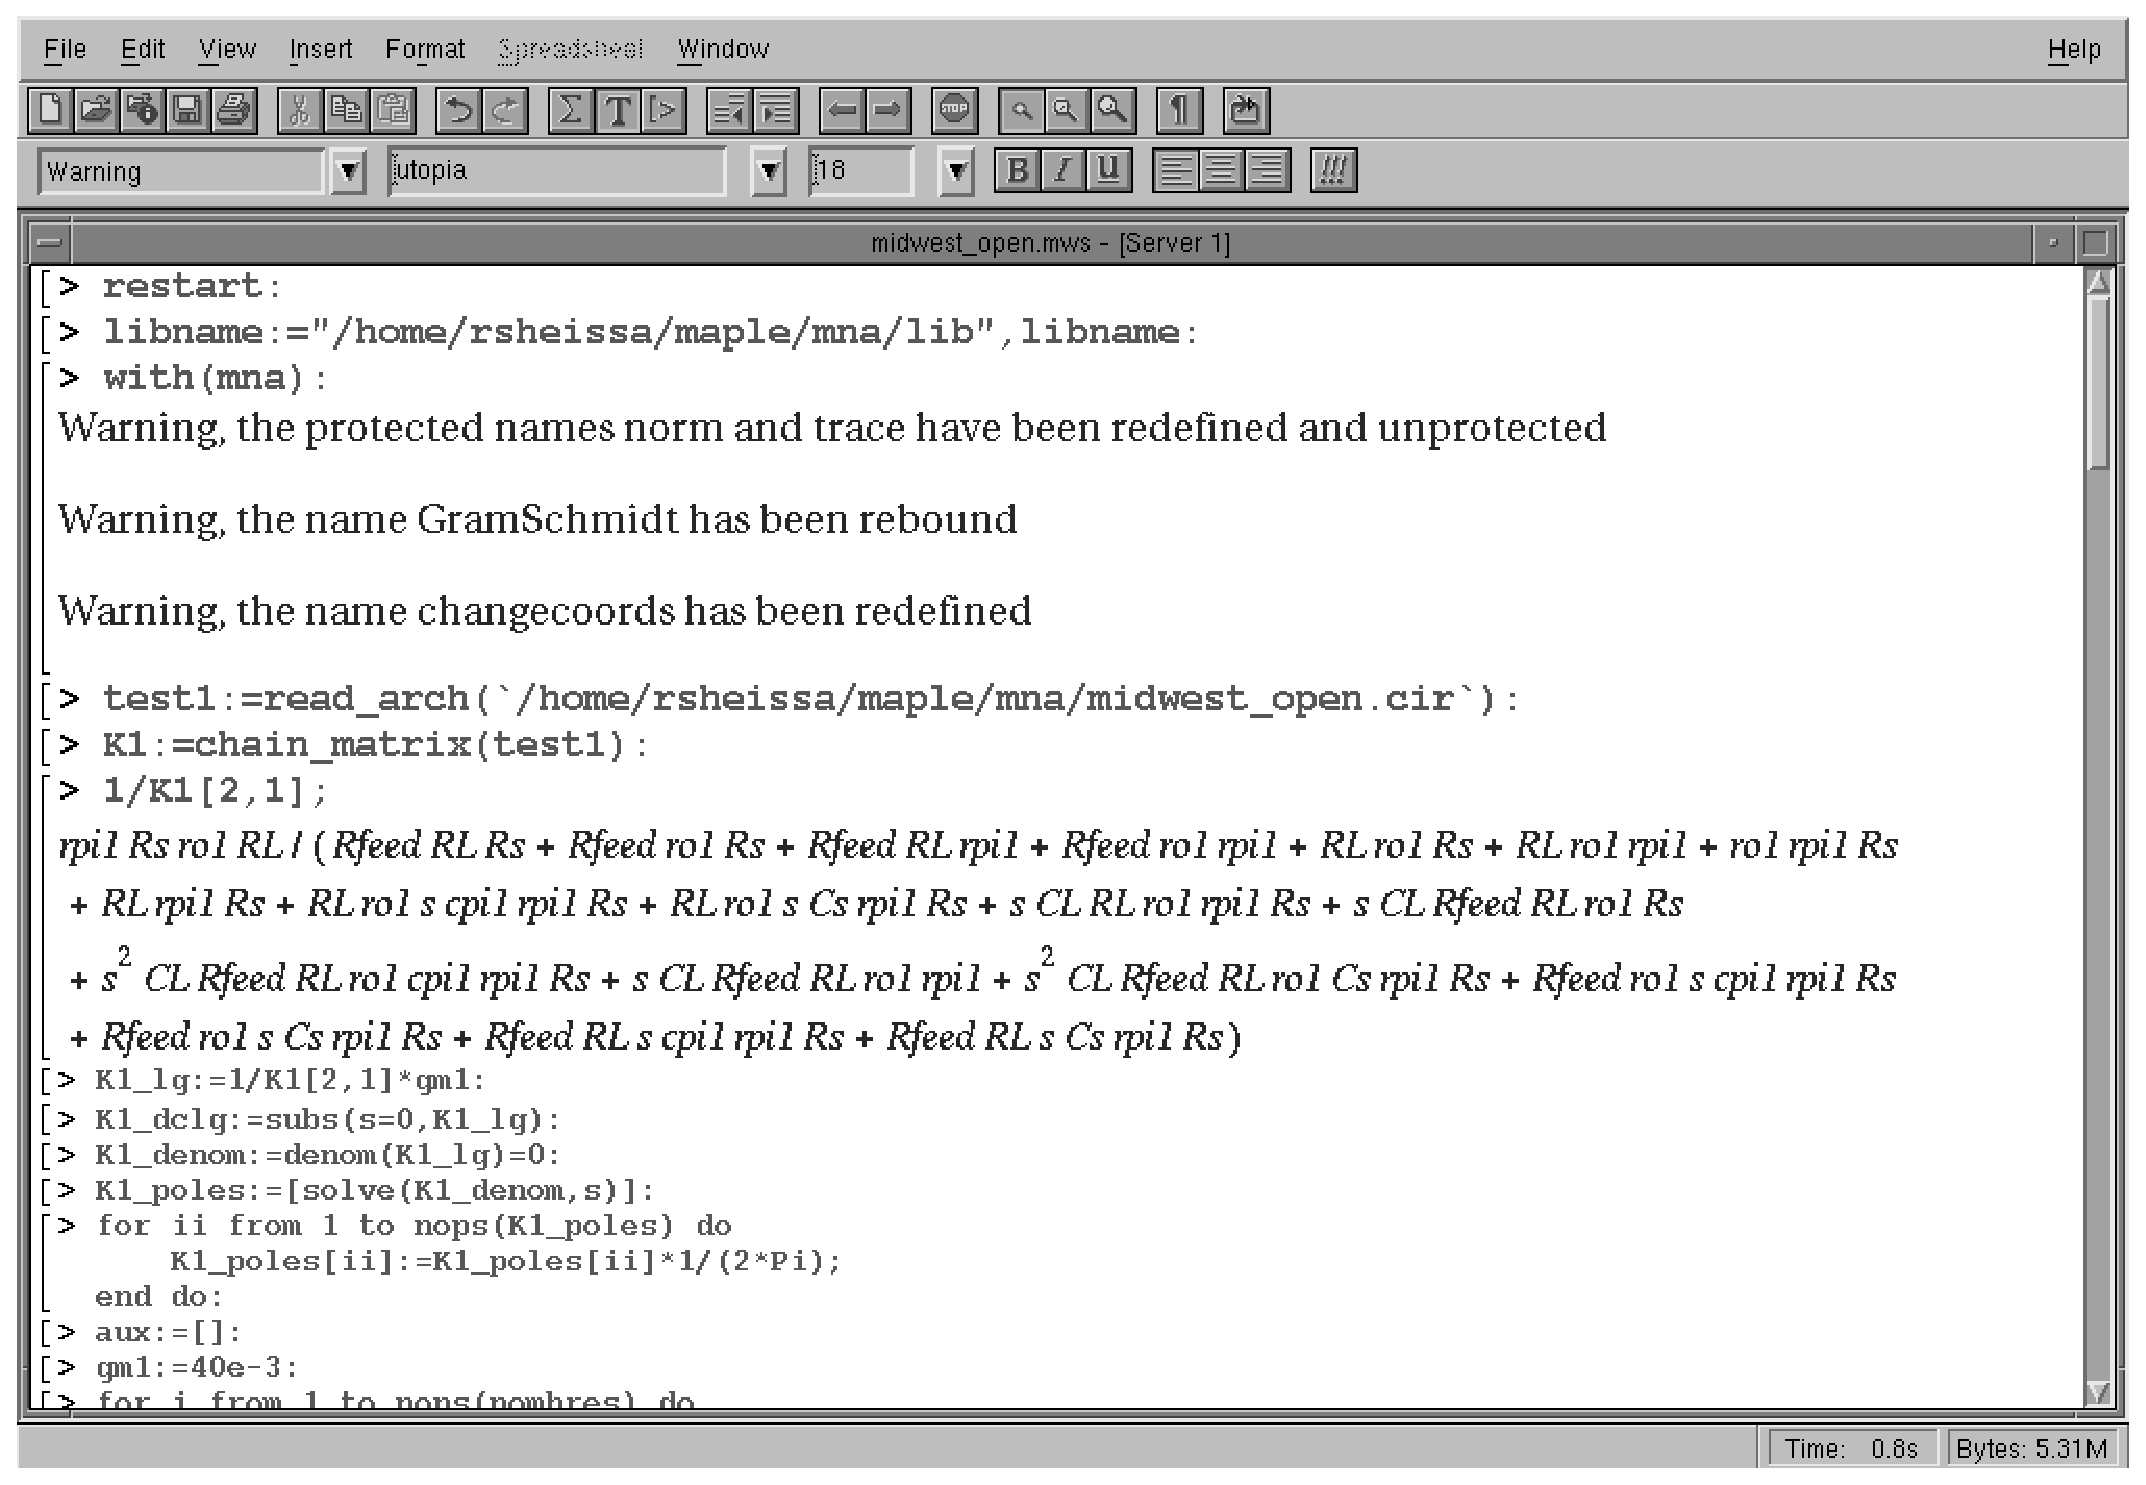
\includegraphics[scale=.24]{figures/maple_1.eps}
	\caption{Chain-matrix for Current-Voltage Amplifier.}
	\label{fig:maple_1}
\end{figure}

Opening the loop, poles are located at (Figure \ref{fig:maple_2}).

\begin{figure}[hbtp]
	\centering
	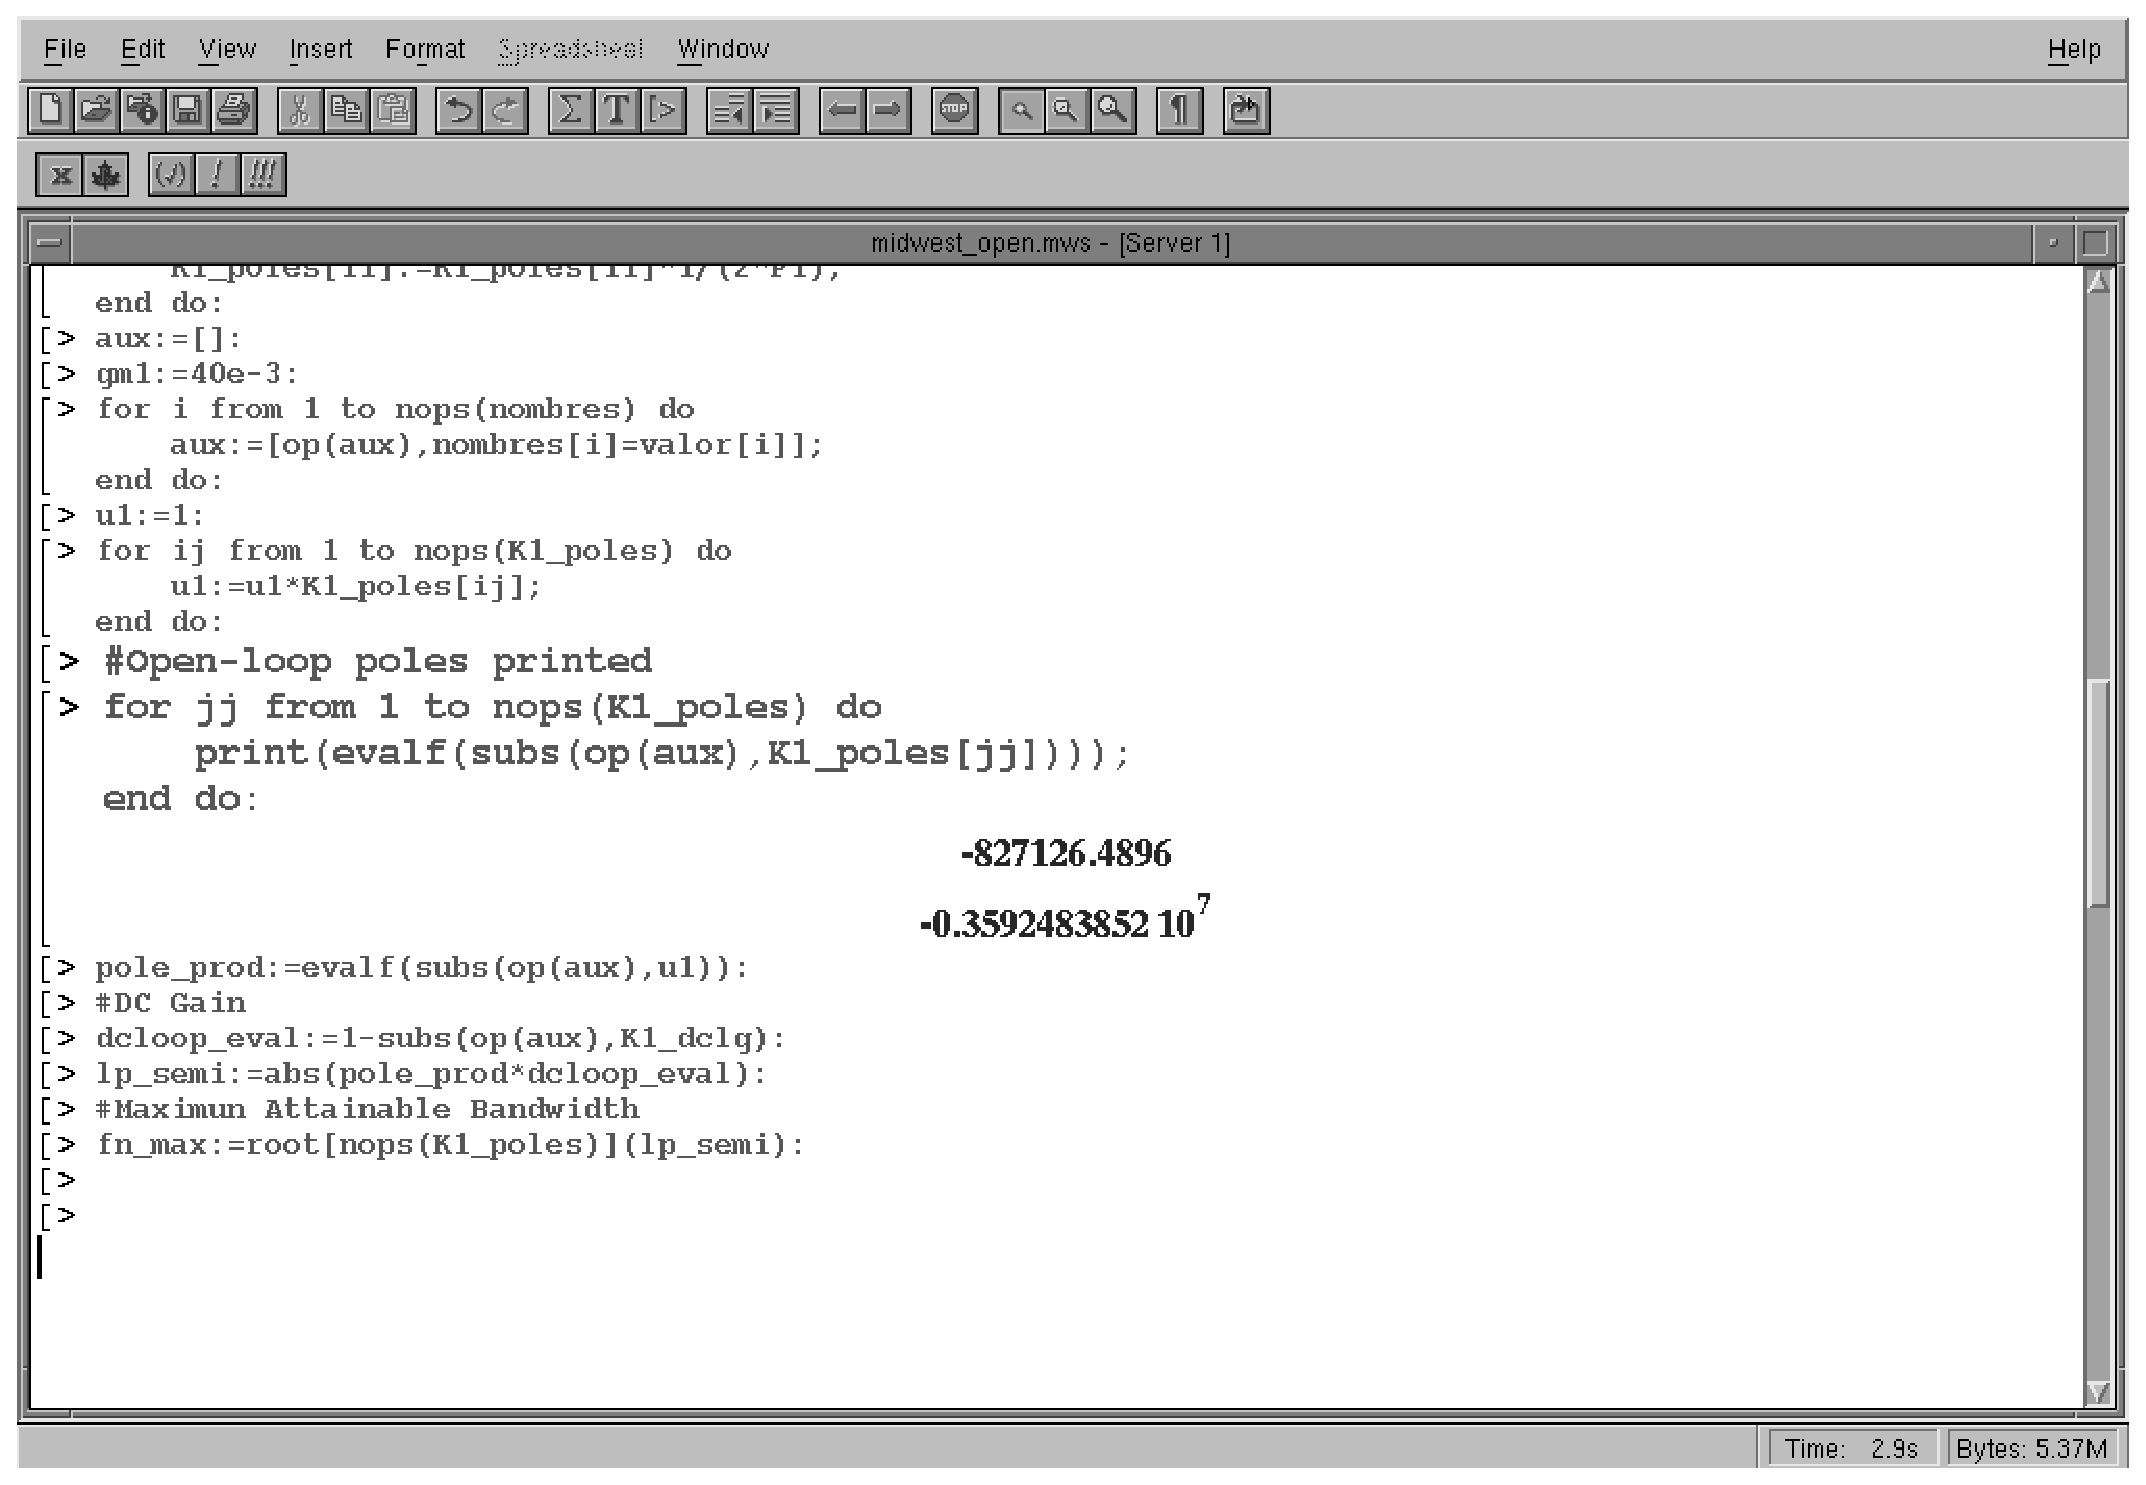
\includegraphics[scale=.24]{figures/maple_2.eps}
	\caption{Poles Calculation Procedure and Display.}
	\label{fig:maple_2}
\end{figure}

This tool finds that resistor broad-banding is able to move the poles of the circuit into a Butterworth position (Figure \ref{fig:maple_3}). These are the values found:

\begin{figure}[hbtp]
	\centering
	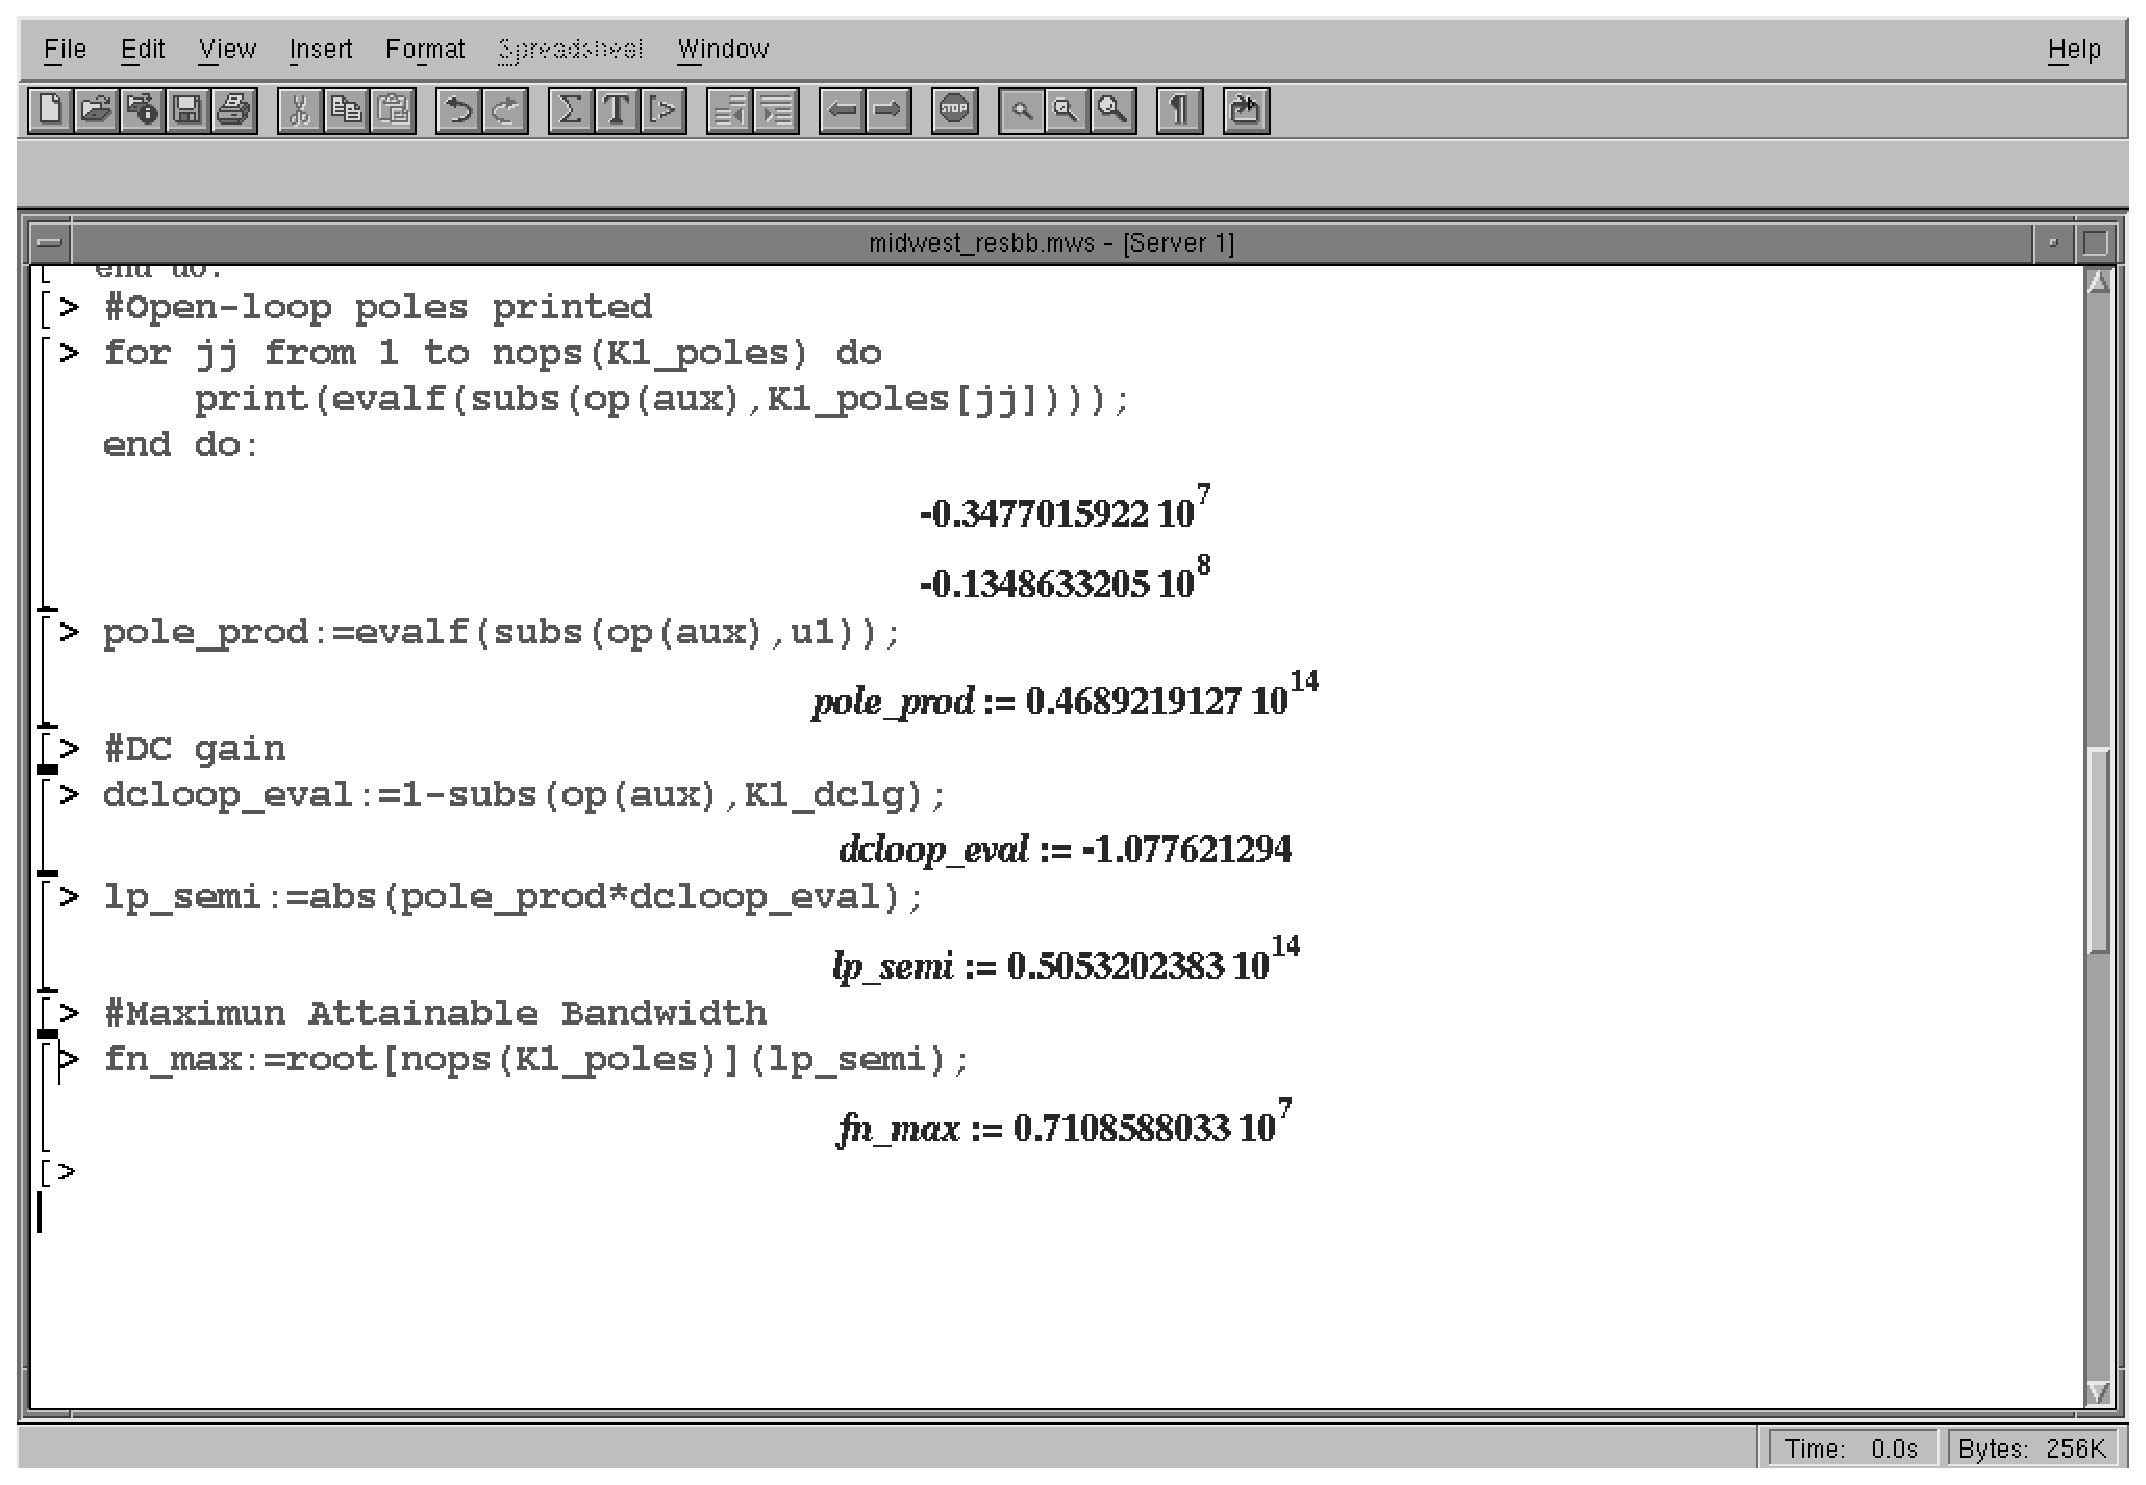
\includegraphics[scale=.24]{figures/maple_3.eps}
	\caption{Results of the Resistor Broad-banding Calculation Procedures.}
	\label{fig:maple_3}
\end{figure}

\begin{itemize}
\item Pole= -3477015.922
\item Pole= -13486332.05
\item DC loop gain= -1.077621294
\item Maximum attainable bandwidth= $7108588.033\text{E}^7$
\end{itemize}

\noindent{It can provide a Butterworth characteristic when the loop is closed.}

By means of a simulation in hspice \cite{hspice} is verified that poles are placed at a Butterworth position. The results are:

\begin{itemize}
\item Pole= $-8.4817\text{E}^6+8.5075\text{E}^6\text{j}$
\item Pole= $-8.4817\text{E}^6-8.5075\text{E}^6\text{j}$
\end{itemize}

\noindent{calculating the angle it gives $45.09^{o}$ for a $R_{br}=122\,\Omega$. The schematic (Figure \ref{fig:transimp_3}) show where this resistor is placed.}

\begin{figure}[hbtp]
	\centering
	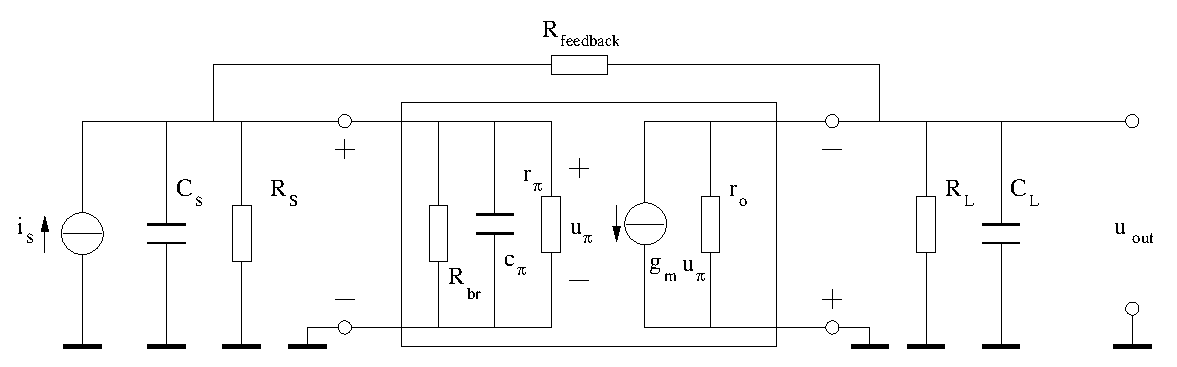
\includegraphics[scale=.45]{figures/transimp_3.eps}
	\caption{Implementation of Resistive Broad-banding.}
	\label{fig:transimp_3}
\end{figure}


\section{Conclusion}
It has been shown that by applying the theory provided by the structured design method is possible to verify if a design can accomplish the bandwith spec once the noise and distortion stages are completely designed. A CAD tool based on the Maple program has been developed in order to verify if the amplifier design can accomplish the bandwidth behavior for what it was designed.  In case that design does not reach the desired bandwidth or its poles are not in a Butterworth distribution, the program has various procedures to make it fulfill specs. These procedures resort to various techniques and concepts. The Loop-Pole product ({\it LP}) makes easier to measure the bandwidth capability of an amplifier. If the LP product is lower, it is impossible to reach a desired bandwidth. There are two techniques in order to increase the LP product. Once the BW spec is fulfilled the position of the poles is the next concern. Four frequency compensation techniques can be applied. If after frequency compensations or LP product increase there is not a satisfactory pole placement or a high LP value, the need the re-design the amplifier becomes a priority. 

\section*{Acknowledgment}
Roberto Casta\~neda Sheissa is holder of a scholarship from CONACyT M\'exico under contract 118652/120341. This work has been supported by a CONACyT M\'exico research project under grant 42588-Y.


\bibliography{bib/midwest}


% that's all folks
\end{document}


